\section*{Appendix: Detailed Results}
\label{app:start}

This appendix collects proof and algorithm detail, the kernel-dual table, the per-dataset and
per-scene numbers behind Table~\ref{tab:real}, and the systems, baseline, and ablation detail.

\subsection*{A. Proofs, derivation notes, and the backward algorithm}
\label{app:proofs}
\label{app:backward}

The complete proofs of Lemmas~\ref{lem:brdual}--\ref{lem:weights},
Theorems~\ref{thm:gnc}--\ref{thm:rhs}, Propositions~\ref{prop:signflip}--\ref{prop:bound}, the
Schur-complement identity, the Riemannian Hessian formula, and the existence construction are
maintained in the project theory notes (\texttt{theory/proofs.md} and
\texttt{theory/derivations.md}); numerical checks are in \texttt{verify/}. The main text states the
results and the proof sketches; in particular:

\begin{itemize}
\item \emph{Lemma~\ref{lem:brdual}}: $w\mapsto we+\psi_\mu(w)$ is strictly convex on $(0,1]$ with
  stationary point $w^*$; substituting $w^*$ recovers $\rho_\mu(e)$, and the box constraint is a
  Cartesian product, so the multi-observation minimum is separable.
\item \emph{Lemma~\ref{lem:schur}}: differentiating the joint objective in $(z,w)$ gives $H_J$;
  eliminating $\delta w$ with $\psi''(w_i^*)=-1/\rho''(e_i^*)>0$ gives
  $H_{\mathrm{rob}}=H_{\mathrm{IRLS}}+\Delta H_{\mathrm{redesc}}$.
\item \emph{Lemma~\ref{lem:hessian}}: for $f\in C^2(\mathcal{M})$ the Euclidean Hessian restricted
  to the tangent space differs from the Riemannian Hessian by the second fundamental form, which for
  the unit sphere contributes $-(\mathbf{q}^\top G_q)\diag(I_4,0_3)$ \cite{absil2008}. For 3D--3D,
  $g_{i,q}^E=2J_i^\top W_i\mathbf{r}_i$ and $J_i\mathbf{q}=2\mathbf{u}_i$, hence
  $\lambda_i=\mathbf{q}^\top g_{i,q}^E=4\mathbf{u}_i^\top W_i\mathbf{r}_i$. The $W_i(\theta)$
  extension adds $2\mathbf{r}_i^\top(\partial W_i/\partial\theta)\mathbf{r}_i$ to
  $\partial e_i/\partial\theta$ and leaves the Hessian at fixed $W_i$ unchanged.
\item \emph{Proposition~\ref{prop:existence}}: the sign of
  $\Phi(t)=\sum_i2\rho'(e_i)(t-y_i)$ is evaluated at $t=0$ and $t=Kc^4/d^3$ for $d=y_2-y_1$, with
  $H_{\mathrm{rob}}\to\lambda_\parallel(0)=2>0$ as $d\to\infty$.
\item \emph{Proposition~\ref{prop:bound}}: the constants follow from
  $\|\partial\Phi/\partial\mathbf{y}_i\|_F\le Cc^4/(c^2+e_i)^2$,
  $\lambda_{\min}(H_{\mathrm{rob}})\ge\mu_0$, $\|\mathbf{r}_i\|^2=e_i$ for $W_i=I$, and
  $\|\rho'(e_i)g_i\|\le2\overline wc^4/\|\mathbf{r}_i\|^3$.
\end{itemize}

\begin{algorithm}[t]
\caption{Exact backward pass (implicit differentiation of the robust fixed point)}
\label{alg:backward}
\footnotesize
\begin{algorithmic}[1]
\Require upstream gradient; cached $z^*,w^*,e^*$
\For{$i=1$ to $N$}
  \State compute $\mathbf{u}_i,\mathbf{r}_i,J_i,g_i^E\in\mathbb{R}^7,H_i^E\in\mathbb{R}^{7\times7}$
\EndFor
\State $G\gets\sum_i\rho'_i g_i^E$;\quad
       $H_E\gets\sum_i\big(\rho'_iH_i^E+\rho''_ig_i^Eg_i^{E,\top}\big)$
\State $B_q\gets$ orthonormal basis of $\mathbf{q}^{*\perp}$;\quad $B\gets\diag(B_q,I_3)$
\State $H_{\mathrm{rob}}\gets B^\top H_EB-\lambda_{\mathrm{rob}}\diag(I_3,0_3)$,\quad
       $\lambda_{\mathrm{rob}}=\mathbf{q}^{*\top}G_q$
\State $\mathrm{RHS}\gets\sum_i\rho'_i\,\mathrm{d}g_i/\mathrm{d}\theta
       +\sum_i\rho''_ig_i(\mathrm{d}e_i/\mathrm{d}\theta)^\top$
\State $\mathrm{d}z\gets\mathrm{solve}(H_{\mathrm{rob}},-\mathrm{RHS})$
\State chain $\mathrm{d}z$ back to $(\mathbf{q},\mathbf{t})$ and to the upstream loss
\end{algorithmic}
\end{algorithm}

\begin{figure}[t]
\centering
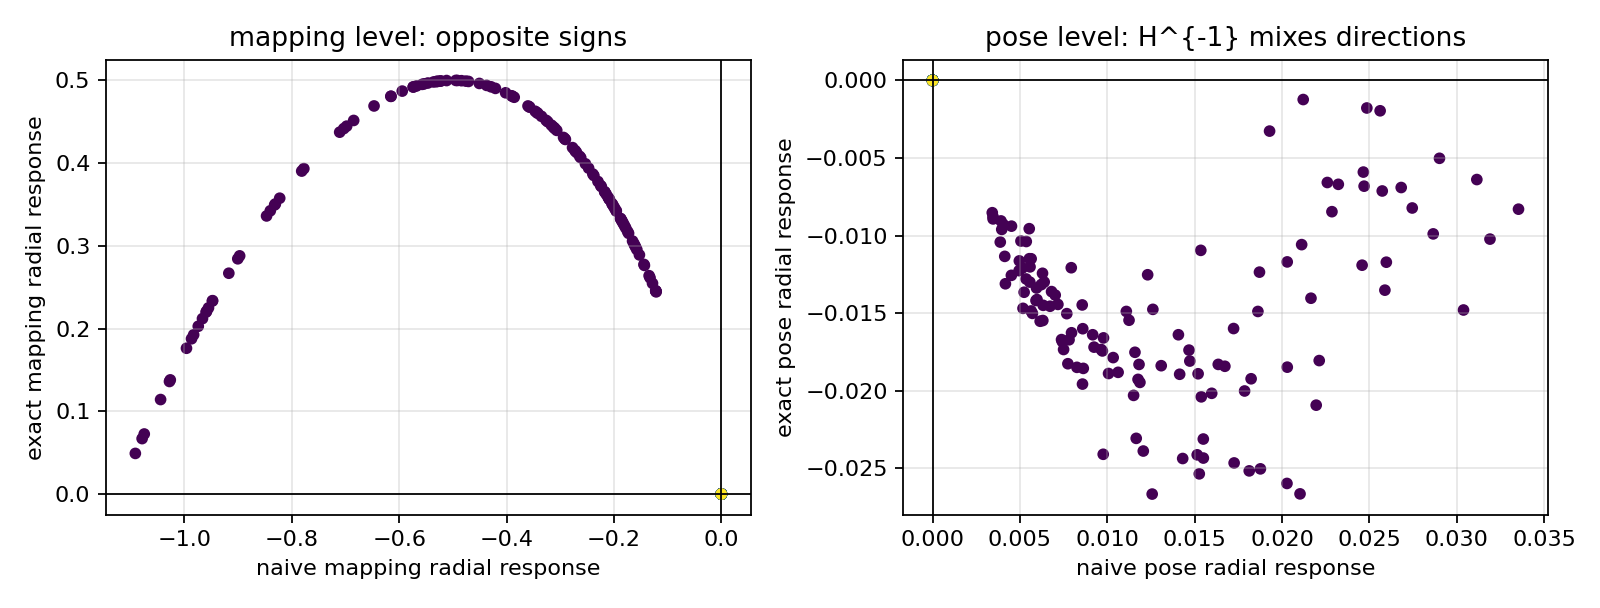
\includegraphics[width=\columnwidth]{gradient_sign.png}
\caption{Numerical sign structure behind Proposition~\ref{prop:signflip}. Left: mapping-level radial
response, exact versus frozen-weight (naive); for $e>c^2/3$ the signs are opposite. Right: pose-level
response after $H_{\mathrm{rob}}^{-1}$; the inverse Hessian mixes directions, so the 6D sign is
numerical.}
\label{fig:sign}
\end{figure}

\subsection*{B. Kernel duals}
\label{app:kernel}

Table~\ref{tab:kernel} lists the BR duals used by the layer, with $a=\mu c^2$. The forward and
backward passes are structurally identical across kernels: only $\rho_\mu'$ and $\psi_\mu''$ change.
TLS has a linear $\psi$ and a non-unique weight at $e=a$; it requires the GNC-TLS schedule rather
than plain bandwidth annealing.

\begin{table}[t]
\caption{Black--Rangarajan duals for the four kernels ($a=\mu c^2$).}
\label{tab:kernel}
\centering
\scriptsize
\setlength{\tabcolsep}{1.4pt}
\begin{tabular}{llll}
\toprule
kernel & $\rho_\mu(e)$ & $w^*=\rho_\mu'(e)$ & $\psi_\mu(w)$ \\
\midrule
Geman--McClure & $ae/(a+e)$ & $(a/(a+e))^2$ & $a(\sqrt{w}-1)^2$ \\
Cauchy & $a\log(1+e/a)$ & $a/(a+e)$ & $a(w-1-\log w)$ \\
Welsch & $a(1-e^{-e/a})$ & $e^{-e/a}$ & $a(1-w+w\log w)$ \\
TLS & $\min(e,a)$ & $1$ if $e<a$, $0$ if $e>a$ & $a(1-w)$ \\
\bottomrule
\end{tabular}
\end{table}

\subsection*{C. Per-dataset results}
\label{app:datasets}

\noindent\textbf{ModelNet40/10.} Table~\ref{tab:modelnet} gives the aggregate numbers. ModelNet10
uses 908 test objects in 10 classes, with OFF meshes resampled to 2048 points; robust-method success
differs from ModelNet40 by at most $2$~pp and median rotation by at most $0.038^\circ$. GNC runs in
$1.7$--$1.9$~ms versus $53.5$--$61.5$~ms for fixed-1000 RANSAC on both datasets.

\begin{table}[t]
\caption{ModelNet object-cloud results under uniform random outliers, 50 trials/cell, $N=100$,
$c=0.05$~m. Entries are success rates; ``fail'' marks collapse.}
\label{tab:modelnet}
\centering
\scriptsize
\setlength{\tabcolsep}{2.5pt}
\begin{tabular}{lcccc}
\toprule
dataset & GNC & RANSAC-1000 & IRLS & Kabsch \\
\midrule
ModelNet40 & $100\%$ $\le70\%$ & $100\%$ & $98$--$100\%$ & fail $\ge50\%$ \\
ModelNet10 & $100\%$ $\le70\%$ & $100\%$ & $98$--$100\%$ & fail $\ge50\%$ \\
\bottomrule
\end{tabular}
\end{table}

\noindent\textbf{3DMatch.} Table~\ref{tab:3dmatch} gives the pooled eight-scene row, the
low/mid/high overlap study, the stricter $0.20$--$0.50$ band, and the two FPFH-front-end audits.
Pooled over all eight official test scenes (20 trials/cell), GNC p50 at $p=0.7$ is $2.26$~ms vs
$62.6$~ms for fixed-1000 RANSAC ($27.7\times$), and the boundary median rotation at $p=0.7$ is
$0.27^\circ$ vs $0.52^\circ$. Per-scene GNC p50 is $2.26$--$2.36$~ms vs $62.1$--$73.4$~ms
($27.4$--$31.1\times$), IRLS is $99\%$ at $70\%$, and coherent outliers collapse at $60$--$70\%$ for
every method ($0\%$). The overlap study selects 24/21/20 pairs for the high/mid/low bins; clean
rotation is $0.18^\circ$/$0.24^\circ$/$0.52^\circ$, yet GNC and RANSAC both stay at $100\%$ at
$p=0.7$ in every bin, with a zero success delta and a $27.7$--$30.4\times$ speedup for $p\ge30\%$.
The low bin still has a median base inlier fraction of $0.95$. The stricter $0.20$--$0.50$
geometric-overlap band (4 low + 2 matched high pairs per scene, 10 trials/cell) has oracle base
inlier $0.953$ (low) / $0.984$ (high) and clean rotation $0.47^\circ$ / $0.19^\circ$; GNC and
RANSAC-1000 are $100\%$ at $p=0.7$, IRLS $92\%$, Kabsch $1\%$. Low overlap reduces the \emph{number}
of usable correspondences, not the oracle inlier fraction. The FPFH front-end (mutual NN plus
pairwise-distance consistency, no GT in matching) reaches natural inlier rates of $80.0\%$ and
$67.8\%$ on the two audited scenes.

\begin{table*}[t]
\caption{3DMatch detail. Oracle correspondences use GT-mapped nearest neighbours on real overlapping
fragments; FPFH rows use a hand-crafted front-end with no GT in matching. ``bnd'' = boundary
outliers.}
\label{tab:3dmatch}
\centering
\scriptsize
\setlength{\tabcolsep}{2.2pt}
\begin{tabular}{lcccccc}
\toprule
setting & pairs/trials & clean rot & GNC & RANSAC-1000 & Kabsch & speedup \\
\midrule
pooled 8 test scenes, random & 8 pairs/scene, 20 trials/cell & --- & $100\%$ $\le70\%$ & $100\%$ & --- & $27.7\times$ @$70\%$ \\
pooled 8 test scenes, bnd.\ @$70\%$ & 8 pairs/scene, 20 trials/cell & --- & $0.27^\circ$ & $0.52^\circ$ & --- & --- \\
overlap high & 24 pairs & $0.18^\circ$ & $100\%$ @$0.7$ & $100\%$ & --- & $27.7$--$30.4\times$ \\
overlap mid & 21 pairs & $0.24^\circ$ & $100\%$ @$0.7$ & $100\%$ & --- & $27.7$--$30.4\times$ \\
overlap low & 20 pairs & $0.52^\circ$ & $100\%$ @$0.7$ & $100\%$ & --- & $27.7$--$30.4\times$ \\
strict $0.20$--$0.50$ band & 4 low + 2 high pairs/scene, 10 trials/cell & $0.47^\circ$ / $0.19^\circ$ & $100\%$ @$0.7$ & $100\%$ & $1\%$ & --- \\
FPFH audit 1 & natural inliers $80.0\%$ & --- & $100\%$ & $100\%$ & $100\%$ & --- \\
FPFH audit 2 & natural inliers $67.8\%$ & --- & $100\%$ & $97\%$ & $83\%$ & --- \\
\bottomrule
\end{tabular}
\end{table*}

\noindent\textbf{KITTI.} Table~\ref{tab:kitti} collects the raw-drive and odometry rows. For the raw
drives, ego motion comes from OXTS (Mercator + roll/pitch/yaw) mapped to Velodyne with
\texttt{calib\_imu\_to\_velo}; direction is verified (drive 0001 correct NN $0.100$--$0.123$~m vs
inverse $0.143$--$0.183$~m; drive 0002 $0.108$--$0.140$~m vs $0.136$--$0.269$~m). Drive 0002
reproduces the drive-0001 random and boundary tables exactly, keeps the coherent transition (at
$50\%$ GNC $40\%$ vs $35\%$, IRLS $30\%$ vs $45\%$; both chance-level), and gives the
$\sim21$--$23\times$ speedup. A threshold sweep keeps GNC at $100\%$ for
$c\in\{0.15,0.25,0.35\}$, with $c=0.25$ matching the $\sim0.10$~m point spacing. For odometry, only
the 32--33 touched frames per sequence were range-fetched from the 84.8~GB official archive, so all
11 sequences 00--10 are represented. On the eight added sequences (10 trials/cell) success is
$100\%$ for GNC and RANSAC-1000 at $p=0.7$ except seq~08 ($80\%$ at $p=0$ and $p=0.3$; RANSAC
$100\%$); pooled over 11 sequences success is $99/99/100/100\%$ at $p=0/0.3/0.5/0.7$, and the
fixed-RANSAC/GNC runtime ratio is $22.4\times$ at $p\ge0.3$. The 00/05/07 subset gives the
failure-mode detail: all 18 direction checks pass (fwd NN $0.053$--$0.114$~m vs inverse
$0.104$--$0.430$~m), random success is $100\%$ through $70\%$, pooled GNC $2.8$~ms vs $73.7$~ms
($26.3\times$), coherent collapse at $p=0.6$ (at $p=0.5$ GNC $53\%$, IRLS $38\%$, RANSAC $0\%$),
boundary $0.067^\circ$ vs $0.143^\circ$, and across $|\mathbf{t}|=0.09$--$9.62$~m and gaps
$1/2/4/8$ (171 paired cells) GNC is never below RANSAC. The exact-pose clean floor
($0.042$--$0.057^\circ$) is not lower than the OXTS raw drives ($0.030$--$0.039^\circ$), so LiDAR
sampling/voxelization dominates it.

\begin{table*}[t]
\caption{KITTI raw drives and odometry, $N=300$, $c=0.25$~m, 20 trials/cell (added sequences 10
trials/cell). Random-outlier success is $100\%$ for GNC and fixed-1000 RANSAC through $70\%$ except
seq~08.}
\label{tab:kitti}
\centering
\footnotesize
\setlength{\tabcolsep}{3pt}
\begin{tabular}{lcccccc}
\toprule
sequence & frames/pairs & GNC p50 & RANSAC p50 & speedup & coh.\ @$50\%$ & bnd.\ rot \\
\midrule
raw 0001 & 108 frames, 10 pairs & $2.7$--$2.8$~ms & $61$--$64$~ms & $\sim22\times$ & $0\%$ all & $0.07$--$0.09^\circ$ \\
raw 0002 & 77 frames, 10 pairs & $2.7$--$2.8$~ms & $61$--$64$~ms & $\sim21$--$23\times$ & $40/35/30/45\%$ & $0.07$--$0.09^\circ$ \\
odom 00--10 & 33 frames each, pooled & $2.8$~ms & $73.7$~ms & $22.4\times$ & seq~08 $80\%$ @$p\le0.3$ & --- \\
odom 00/05/07 & 33 frames each & $2.8$~ms & $73.7$~ms & $26.3\times$ & $53/38/0\%$ & $0.067/0.143^\circ$ \\
\bottomrule
\end{tabular}
\end{table*}

\noindent\textbf{In-The-Dark.} Table~\ref{tab:inthedark} gives the daylight runs and the night
windows. The composed official GT was validated by stereo reprojection on disjoint pairs: forward
medians $0.65$~px (run\_000002) and $0.52$~px (run\_000012), versus $18.1/27.9$~px inverse,
$9.5/14.7$~px identity, and $21.5/31.3$~px unconjugated. All checks pass (512$\times$384 images,
left/right row alignment $0.56$--$0.58$~px). The archive is 905~MB but only the 315{,}463-byte
transform file was range-fetched (CRC verified); the night zips (2.6--2.76~GB) were not downloaded,
and only the touched windows were fetched. The motion-matched daylight control (run\_000002 start
757, $|\mathbf{t}|=0.21$~m, rot $0.54^\circ$) gives $85.9\%$ inliers and $0.121^\circ/0.007$~m;
median depth is $4.5$~m at night vs $6.7$--$7.2$~m by day, so the night inlier rate is a geometry
effect rather than a property of SIFT in low light.

\begin{table*}[t]
\caption{UTIAS In-The-Dark: two daytime runs (15 consecutive pairs each) and two night-window
prefixes (10 pairs each); hand-written SIFT+StereoSGBM front-end, no training. GT reprojection
columns are median px (fwd / inverse / identity / unconjugated vehicle frame).}
\label{tab:inthedark}
\centering
\footnotesize
\setlength{\tabcolsep}{3pt}
\begin{tabular}{llcccccc}
\toprule
run & pairs & inliers & rot & trans & succ.\ @$0.1$~m & Kabsch & GT reproj \\
\midrule
day run\_000002 & 15 & $79.4\%$ & $0.078^\circ$ & $0.020$~m & $100\%$ & $47\%$ & $0.65/18.1/9.5/21.5$ \\
day run\_000012 & 15 & $88.5\%$ & $0.092^\circ$ & $0.010$~m & $100\%$ & $40\%$ & $0.52/27.9/14.7/31.3$ \\
night run\_000017 & 10 & $96.0\%$ & $0.135^\circ$ & $0.011$~m & $100\%$ & --- & --- \\
night run\_000018 & 10 & $97.1\%$ & $0.150^\circ$ & $0.011$~m & $100\%$ & --- & --- \\
night sparse & 10 & $84.3\%$ & $0.197^\circ$ & $0.015$~m & --- & --- & --- \\
day control & 10 & $85.9\%$ & $0.121^\circ$ & $0.007$~m & --- & --- & --- \\
\bottomrule
\end{tabular}
\end{table*}

\noindent\textbf{KITTI stereo front end.} Thirty frame pairs of drive 0001 with SIFT + sub-pixel +
StereoSGBM on rectified \texttt{image\_02/03} ($b=0.5327$~m) give a natural inlier rate of $17.8\%$
at $c=0.5$~m with 890 correspondences/pair. GNC/IRLS recover rotation to $0.052^\circ$ against a
GT-inlier floor of $0.071^\circ$, but translation is $0.70$~m median versus $1.92$~m motion and a
$0.239$~m floor; no method attains $0.1$~m or $0.25$~m success. GNC is $19.3\times$ faster than
fixed-1000 RANSAC (4.21 vs 81.3~ms). The stereo-vs-LiDAR depth ratio is $1.000$--$1.061$ over
3--60~m, ruling out a disparity-scale error; the residual is a coherent forward-translation
under-estimate ($0.63$--$0.73$) from front-end, occlusion, and dynamic bias.

\subsection*{D. Systems, batching, and the inner solver}
\label{app:systems}

A vectorized NumPy GNC over $(B,N,3)$ reproduces the loop to rotation $\le1.1\times10^{-14}$ and
translation $\le1.2\times10^{-15}$ with identical $\mu$-schedules. At $B=32,N=100$ the batch p50 is
$8.5$~ms vs $56.2$~ms for the loop ($6.60\times$); at $B=8$ the speedup is $2.95\times$ ($N=100$)
and $3.27\times$ ($N=500$); $B=1$ is slower ($0.54\times$), so the loop remains the right choice for
single instances.

A $4\times4$ Davenport/Horn inner solver \cite{horn1987} is numerically equivalent to weighted
Kabsch (max $\|R_d-R_k\|_F=1.07\times10^{-14}$, max cost excess $9.4\times10^{-16}$) but its
runtime is better only at large $N$: p50 ratio $0.94\times$ ($N=20$), $1.02\times$ ($N=100$),
$1.28\times$ ($N=500$), geometric mean $1.07\times$. It is a large-$N$ option rather than a
default $N=100$ gain.

\subsection*{E. External baselines (synthetic only)}
\label{app:baselines}

Theseus 0.2.3 (dense Cholesky; \texttt{scikit-sparse} unavailable without SuiteSparse headers)
solves the same per-point GM objective; its Jacobian matches finite differences at
$1.09\times10^{-10}$ relative error and its GM cost agrees exactly. With GT initialization Theseus-GM
succeeds $100\%$ at all $p$ (a local-basin check, not global recovery); with random initialization it
succeeds $100/80/55/25\%$ at $p=0/0.3/0.5/0.7$, p50 $358$--$670$~ms. On the same 20 instances GNC-GM
is $100\%$ at every $p$ at $1.7$~ms, RANSAC-adaptive is $100\%$ at $0.2$--$14.1$~ms, and Kabsch
fails for $p\ge0.3$. The 20-trial Wilson intervals for Theseus random-init at $p=0.3$
([0.58,0.92]) overlap GNC's 20/20 ([0.84,1.00]), so that gap is not significant; $p=0.5/0.7$ are
separated (Table~\ref{tab:baselines}).

\begin{table}[t]
\caption{Synthetic external baselines, 20 instances per $p$; success (\%) at $p=0/0.3/0.5/0.7$ and
p50 time.}
\label{tab:baselines}
\centering
\footnotesize
\setlength{\tabcolsep}{3pt}
\begin{tabular}{lcccc}
\toprule
method & $p=0$ & $0.3$ & $0.5$ & $0.7$ / time \\
\midrule
Theseus-GM, GT init & 100 & 100 & 100 & 100 \\
Theseus-GM, rand.\ init & 100 & 80 & 55 & 25 / 358--670~ms \\
GNC-GM & 100 & 100 & 100 & 100 / 1.7~ms \\
RANSAC-adaptive & 100 & 100 & 100 & 100 / 0.2--14.1~ms \\
Kabsch & 100 & fail & fail & fail \\
SDPRLayers+SCS & 100 & fail & fail & fail / 8.5--13.4~ms \\
\bottomrule
\end{tabular}
\end{table}

SDPRLayers+SCS (fresh \texttt{utiasASRL/sdprlayer} at cb3aed2, SCS, 208 forwards) is numerically
available: $0/208$ SCS exceptions, $8.5$--$13.4$~ms. It succeeds at $p=0$ but fails at $p\ge0.3$, as
expected without a robust kernel. With $W_i=I$ and unit weights its objective equals Kabsch: 80
paired trials give max $|\Delta R|=1.5\times10^{-5}$~deg and max $|\Delta t|=1.3\times10^{-9}$~m.
This row validates forward correctness and availability; a distinct SDPR requires non-identity
$W_i$ (e.g.\ POLI) or RANSAC. BPnP is 3D--2D PnP only, Pyatov \emph{et al.} is two-view 2D--2D, and
POLI is a per-point geometry estimator, so none is a direct 3D--3D baseline.

\subsection*{F. Ablations}
\label{app:ablations}

\noindent\textbf{Kernel.} With the same weighted-Kabsch inner and schedule, GM, Cauchy, and Welsch
are all $100\%$ on random and boundary outliers through $70\%$ (Table~\ref{tab:kernelabl}). GM has
the lowest boundary median rotation at $50$--$70\%$ ($0.199/0.229/0.340^\circ$ vs Cauchy
$0.241/0.264/0.370^\circ$ and Welsch $0.220/0.268/0.392^\circ$). There is no evidence to switch the
default.

\begin{table}[t]
\caption{Kernel ablation: boundary median rotation (deg) at $p=0.5/0.6/0.7$; all kernels are
$100\%$ on random and boundary outliers through $70\%$.}
\label{tab:kernelabl}
\centering
\footnotesize
\setlength{\tabcolsep}{4pt}
\begin{tabular}{lccc}
\toprule
kernel & $p=0.5$ & $p=0.6$ & $p=0.7$ \\
\midrule
GM (default) & $0.199$ & $0.229$ & $0.340$ \\
Cauchy & $0.241$ & $0.264$ & $0.370$ \\
Welsch & $0.220$ & $0.268$ & $0.392$ \\
\bottomrule
\end{tabular}
\end{table}

\noindent\textbf{GNC schedule.} Sweeping $\gamma\in\{1.2,1.4,1.7,2.0\}$, the $\mu_0$ multiplier
$\{0.5,1,4\}$ and polish steps $\{0,5,10\}$ gives $100\%$ success and identical median rotation at
$p=0.3/0.5/0.7$; $\gamma=2.0$ is $1.04$--$1.79\times$ faster than the default, $\gamma=1.2$ is
$1.47$--$2.49\times$ slower. The default is conservative rather than uniquely optimal.

\noindent\textbf{RANSAC strength.} A stronger LO-RANSAC (MSAC score, up to five local refit/re-score
rounds, 0.999 adaptive stop, cap 1000) ties GNC on accuracy (median rotation difference
$\le0.006^\circ$) but is $1.03$--$1.52\times$ slower than plain adaptive RANSAC at every $p$, because
the final consensus refit is already the same estimator.

\noindent\textbf{Anisotropic $W_i$.} With a correct 6-DoF Gauss--Newton inner solve on
Cholesky-whitened residuals, $W_i=I$ matches Kabsch to $5.3\times10^{-13}$. Scalar weighted Kabsch
is not exact for anisotropic $W_i$: its objective ratio at converged GM weights is
$1.002$--$1.007$ (diagonal) and $1.035$--$1.088$ (full SPD), with a single-trial maximum of $3.80$.
Under the isotropic synthetic noise, however, anisotropic $W_i$ is a misspecified model: full-$W$
GNC has a paired median rotation change of $+0.055$ to $+0.124^\circ$, is better on only
$8$--$32\%$ of trials, and has $92\%$ success at $p=0.7$ (identity: $100\%$). The exact inner solve
is $4.9$--$23\times$ slower than scalar Kabsch. The nonlinear inner solve is therefore appropriate
when $W_i$ is genuinely anisotropic, while anisotropy does not improve accuracy on this isotropic
data.

\subsection*{G. End-to-end boundary diagnostic}
\label{app:e2e}

A GT-supervised test-time refinement updates only the injected boundary observations for 20 Adam
steps. At $p=0.5$, lr $10^{-3}$, the exact gradient reaches a final loss of $1.90\times10^{-6}$ vs
$1.66\times10^{-5}$ for naive (paired median ratio $0.071$, a $14\times$ reduction; exact lower on
$10/10$ seeds) and rotation error $0.029^\circ$ vs $0.087^\circ$; at $p=0.7$ the median ratio is
$0.059$ ($17\times$) and exact wins $9/10$. The all-points control is not discriminative
($4$--$9/10$, ratio $0.64$--$1.04$). A float64 PyTorch \texttt{autograd.Function} passes
\texttt{gradcheck} at $N=6/8/10$ and agrees with NumPy to $10^{-16}$ in pose; a per-point MLP
refinement (5 seeds, $p=0.4$, 50 Adam steps) reduces median rotation from $0.635^\circ$ to
$0.068^\circ$ for exact vs $0.106^\circ$ for naive (exact wins $4/5$ seeds, median loss ratio
$0.56$), while a disjoint held-out protocol overfits in both arms. This is a controlled test-bed for
the layer implementation rather than a trained real-data system.

The per-coordinate gradient check is exact to
$1.6\times10^{-7}$ / $3.9\times10^{-8}$ / $9.3\times10^{-8}$ relative error, versus $1.42$ / $0.60$ /
$0.38$ for the naive backward. The float64 PyTorch \texttt{autograd.Function} passes
\texttt{gradcheck} at $N=6/8/10$ with maximum absolute error $6$--$8\times10^{-10}$ and maximum
relative error $8\times10^{-9}$--$1.1\times10^{-8}$, except one near-zero element at
$8\times10^{-6}$; the naive backward fails at relative error $1.5$--$1.8$, and the torch port agrees
with NumPy to $10^{-16}$ in pose and $3\times10^{-16}$ in $\mathrm{d}L/\mathrm{d}\mathbf{y}$.

\begin{figure*}[t]
\centering
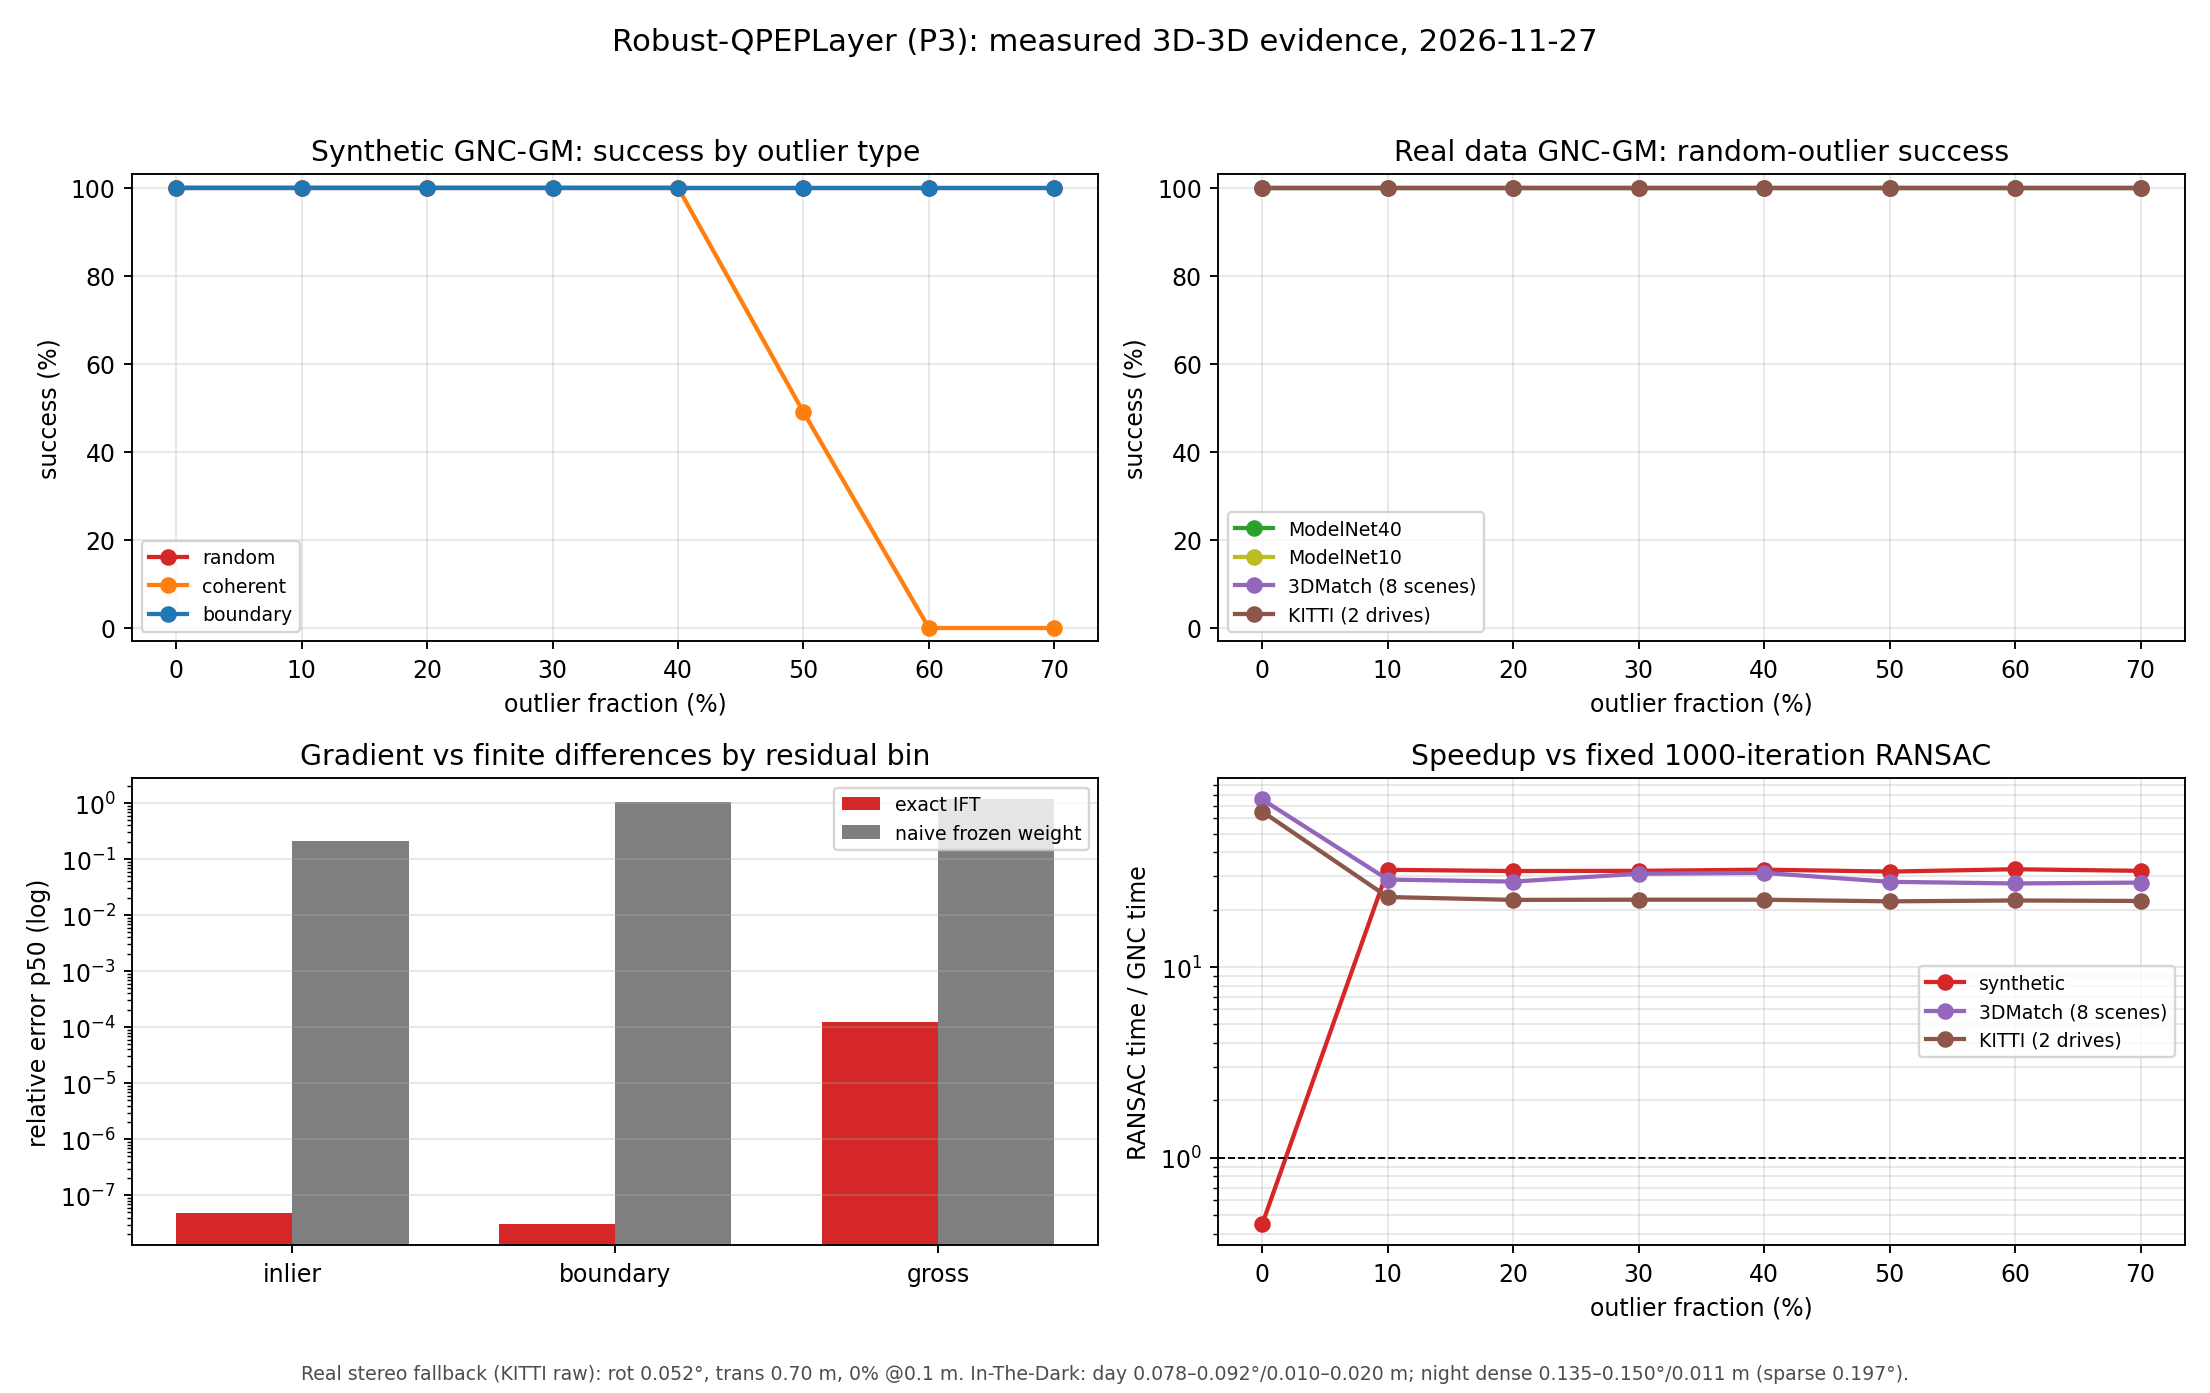
\includegraphics[width=0.92\textwidth]{p3_summary.png}
\caption{Measured 3D--3D evidence. (a) Synthetic GNC-GM success versus outlier fraction for random,
coherent, and boundary outliers: random and boundary stay at $100\%$, coherent collapses once the
outlier transform becomes the global optimum. (b) Real-data random-outlier success for ModelNet40,
ModelNet10, 3DMatch (8 scenes), and KITTI (2 drives); all stay at $100\%$ through $70\%$. (c) 6D
Jacobian relative error (p50, log scale) of exact IFT versus naive frozen weights, by residual bin;
the boundary bin is where freezing fails. (d) GNC p50 runtime advantage over \emph{fixed-1000}
RANSAC on synthetic, 3DMatch, and KITTI data; the dashed line is break-even. The footer reports the
KITTI stereo front end and the In-The-Dark day/night ranges. Success is rotation $<5^\circ$ and
translation $<0.1$~m.}
\label{fig:summary}
\end{figure*}
